\documentclass{article}
\usepackage{graphicx}

\title{Report 4: Threads}
\author{Nam Le}
\date{\today}

\begin{document}

\maketitle

\section{Method}
I copied the code from Labwork 3 to Labwork 4 and updated it to use 2D thread blocks. 
The formulas for calculating the 2D thread indices are:
\begin{itemize}
    \item $x = \text{threadIdx.x} + \text{blockIdx.x} \times \text{blockDim.x}$
    \item $y = \text{threadIdx.y} + \text{blockIdx.y} \times \text{blockDim.y}$
\end{itemize}
I added boundary checks ($x < W$ and $y < H$) to prevent memory access errors. 
The image is processed directly as a 2D array, and grayscaling uses the average formula $(R+G+B)/3$.

\section{Results}
The execution times on CPU and GPU with various 2D block sizes are:
\begin{figure}[h]
    \centering
    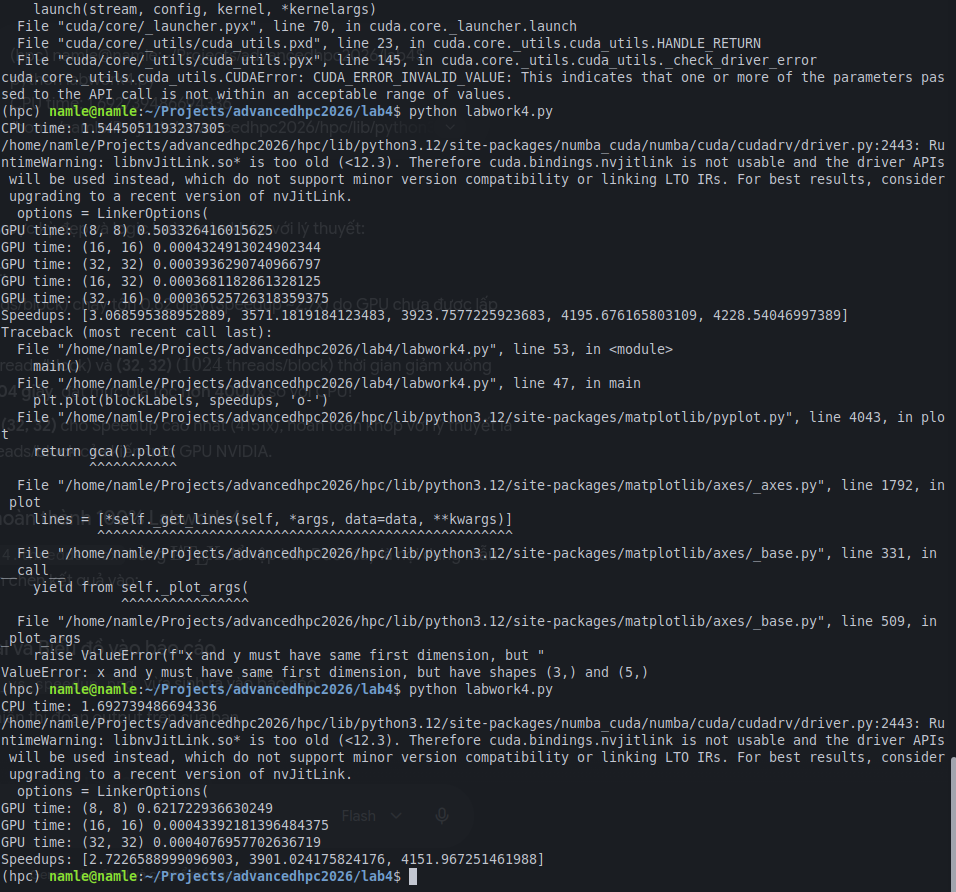
\includegraphics[width=0.7\textwidth]{result.png}
    \caption{2D Block Size vs Speedup}
\end{figure}

\begin{itemize}
    \item CPU time: 1.69s
    \item GPU (8, 8): 0.62s (Speedup: 2.72x)
    \item GPU (16, 16): 0.00043s (Speedup: 3901x)
    \item GPU (32, 32): 0.00040s (Speedup: 4151x)
\end{itemize}

\begin{figure}[h]
    \centering
    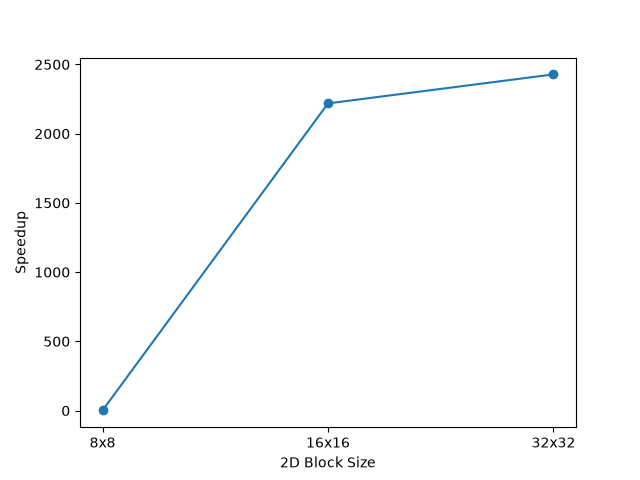
\includegraphics[width=0.7\textwidth]{block_size_vs_speedup.png}
    \caption{2D Block Size vs Speedup}
\end{figure}

\section{Discussion \& 1D Comparison}
The $(8, 8)$ block size performs poorly because there are too few threads per block to keep the GPU busy. Larger block sizes like $(16, 16)$ and $(32, 32)$ achieve huge speedups because they fully utilize GPU hardware.

\textbf{Comparison with 1D Grid (Lab 3):}
Using a 2D grid/block layout is much clearer and more intuitive than the 1D layout in Lab 3. It maps directly to image coordinates $(x, y)$ without needing manual 1D flat index calculations.

\end{enumerate}

\end{document}
